\documentclass{standalone}
\usepackage{tikz}
\usetikzlibrary{patterns, positioning}


\begin{document}
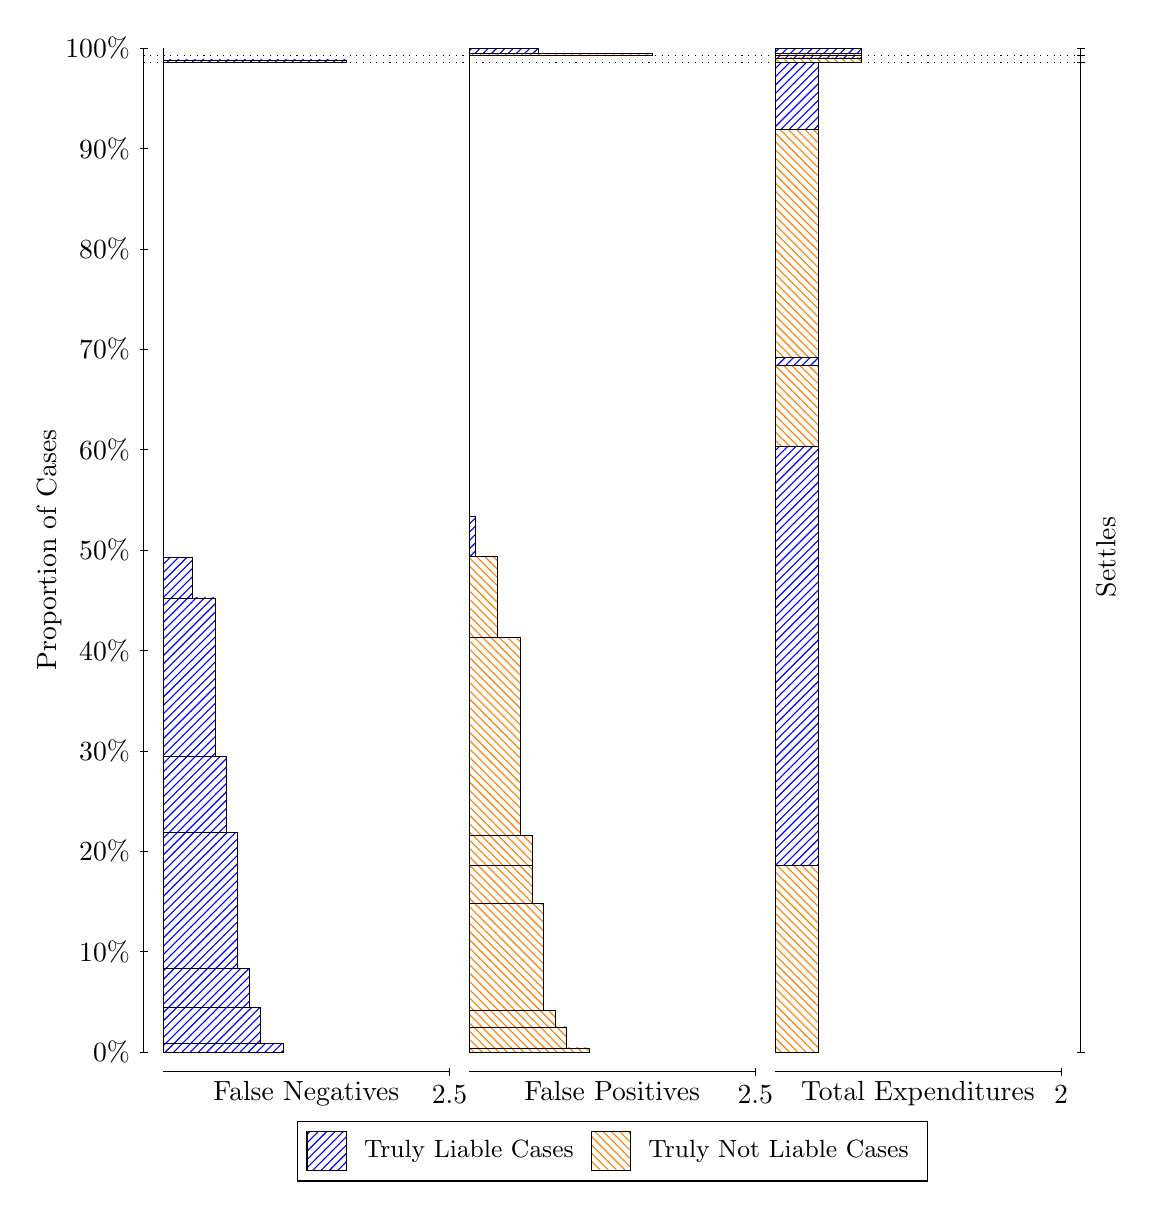
\begin{tikzpicture}
\draw[black, very thin] (1.5,1.75) -- (1.5,14.5);
\node[rotate=90, text=black, anchor=center] at (0.3, 8.125) {Proportion of Cases};
\draw[black, very thin] (1.45,1.75) -- (1.55,1.75);
\node[text=black, anchor=east] at (1.45, 1.75) {0\%};
\draw[black, very thin] (1.45,3.025) -- (1.55,3.025);
\node[text=black, anchor=east] at (1.45, 3.025) {10\%};
\draw[black, very thin] (1.45,4.3) -- (1.55,4.3);
\node[text=black, anchor=east] at (1.45, 4.3) {20\%};
\draw[black, very thin] (1.45,5.575) -- (1.55,5.575);
\node[text=black, anchor=east] at (1.45, 5.575) {30\%};
\draw[black, very thin] (1.45,6.85) -- (1.55,6.85);
\node[text=black, anchor=east] at (1.45, 6.85) {40\%};
\draw[black, very thin] (1.45,8.125) -- (1.55,8.125);
\node[text=black, anchor=east] at (1.45, 8.125) {50\%};
\draw[black, very thin] (1.45,9.4) -- (1.55,9.4);
\node[text=black, anchor=east] at (1.45, 9.4) {60\%};
\draw[black, very thin] (1.45,10.675) -- (1.55,10.675);
\node[text=black, anchor=east] at (1.45, 10.675) {70\%};
\draw[black, very thin] (1.45,11.95) -- (1.55,11.95);
\node[text=black, anchor=east] at (1.45, 11.95) {80\%};
\draw[black, very thin] (1.45,13.225) -- (1.55,13.225);
\node[text=black, anchor=east] at (1.45, 13.225) {90\%};
\draw[black, very thin] (1.45,14.5) -- (1.55,14.5);
\node[text=black, anchor=east] at (1.45, 14.5) {100\%};

\draw[black, very thin] (13.4,1.75) -- (13.4,14.5);
\draw[black, very thin] (13.35,1.75) -- (13.45,1.75);
\node[anchor=west] at (13.35, 1.75) {};
\draw[black, very thin] (13.35,14.319) -- (13.45,14.319);
\node[anchor=west] at (13.35, 14.319) {};
\draw[black, very thin] (13.35,14.405) -- (13.45,14.405);
\node[anchor=west] at (13.35, 14.405) {};
\draw[black, very thin] (13.35,14.5) -- (13.45,14.5);
\node[anchor=west] at (13.35, 14.5) {};

\draw[black, very thin, pattern color=blue, pattern=north east lines] (1.75,1.75) rectangle (3.276,1.856);
\draw[black, very thin, pattern color=blue, pattern=north east lines] (1.75,1.856) rectangle (2.9853,2.321);
\draw[black, very thin, pattern color=blue, pattern=north east lines] (1.75,2.321) rectangle (2.84,2.8103);
\draw[black, very thin, pattern color=blue, pattern=north east lines] (1.75,2.8103) rectangle (2.6947,4.5429);
\draw[black, very thin, pattern color=blue, pattern=north east lines] (1.75,4.5429) rectangle (2.5493,5.5012);
\draw[black, very thin, pattern color=blue, pattern=north east lines] (1.75,5.5012) rectangle (2.404,7.5178);
\draw[black, very thin, pattern color=blue, pattern=north east lines] (1.75,7.5178) rectangle (2.1133,8.0303);
\draw[black, very thin, pattern color=orange, pattern=north west lines] (1.75,8.0303) rectangle (1.75,14.319);
\draw[black, very thin, pattern color=blue, pattern=north east lines] (1.75,14.319) rectangle (4.0753,14.349);
\draw[black, very thin, pattern color=orange, pattern=north west lines] (1.75,14.349) rectangle (1.75,14.405);
\draw[black, very thin, pattern color=orange, pattern=north west lines] (1.75,14.405) rectangle (1.75,14.435);
\draw[black, very thin, pattern color=blue, pattern=north east lines] (1.75,14.435) rectangle (1.75,14.5);
\draw[black, very thin, pattern color=orange, pattern=north west lines] (5.6333,1.75) rectangle (7.1593,1.803);
\draw[black, very thin, pattern color=orange, pattern=north west lines] (5.6333,1.803) rectangle (6.8687,2.0677);
\draw[black, very thin, pattern color=orange, pattern=north west lines] (5.6333,2.0677) rectangle (6.7233,2.2794);
\draw[black, very thin, pattern color=orange, pattern=north west lines] (5.6333,2.2794) rectangle (6.578,3.6386);
\draw[black, very thin, pattern color=orange, pattern=north west lines] (5.6333,3.6386) rectangle (6.4327,4.1178);
\draw[black, very thin, pattern color=orange, pattern=north west lines] (5.6333,4.1178) rectangle (6.4327,4.5013);
\draw[black, very thin, pattern color=orange, pattern=north west lines] (5.6333,4.5013) rectangle (6.2873,7.0142);
\draw[black, very thin, pattern color=orange, pattern=north west lines] (5.6333,7.0142) rectangle (5.9967,8.0392);
\draw[black, very thin, pattern color=blue, pattern=north east lines] (5.6333,8.0392) rectangle (5.706,8.5517);
\draw[black, very thin, pattern color=blue, pattern=north east lines] (5.6333,8.5517) rectangle (5.6333,14.319);
\draw[black, very thin, pattern color=orange, pattern=north west lines] (5.6333,14.319) rectangle (5.6333,14.376);
\draw[black, very thin, pattern color=blue, pattern=north east lines] (5.6333,14.376) rectangle (5.6333,14.405);
\draw[black, very thin, pattern color=orange, pattern=north west lines] (5.6333,14.405) rectangle (7.9587,14.435);
\draw[black, very thin, pattern color=blue, pattern=north east lines] (5.6333,14.435) rectangle (6.5053,14.5);
\draw[black, very thin, pattern color=orange, pattern=north west lines] (9.5167,1.75) rectangle (10.062,4.1178);
\draw[black, very thin, pattern color=blue, pattern=north east lines] (9.5167,4.1178) rectangle (10.062,9.4436);
\draw[black, very thin, pattern color=orange, pattern=north west lines] (9.5167,9.4436) rectangle (10.062,10.469);
\draw[black, very thin, pattern color=blue, pattern=north east lines] (9.5167,10.469) rectangle (10.062,10.575);
\draw[black, very thin, pattern color=orange, pattern=north west lines] (9.5167,10.575) rectangle (10.062,13.471);
\draw[black, very thin, pattern color=blue, pattern=north east lines] (9.5167,13.471) rectangle (10.062,14.319);
\draw[black, very thin, pattern color=orange, pattern=north west lines] (9.5167,14.319) rectangle (10.607,14.376);
\draw[black, very thin, pattern color=blue, pattern=north east lines] (9.5167,14.376) rectangle (10.607,14.405);
\draw[black, very thin, pattern color=orange, pattern=north west lines] (9.5167,14.405) rectangle (10.607,14.435);
\draw[black, very thin, pattern color=blue, pattern=north east lines] (9.5167,14.435) rectangle (10.607,14.5);
\draw[black, dotted] (1.5,14.319) -- (13.4,14.319);
\draw[black, dotted] (1.5,14.405) -- (13.4,14.405);
\draw[black, very thin] (1.75,1.5) -- (5.3833,1.5);
\node[text=black, anchor=north] at (3.5667, 1.5) {False Negatives};
\draw[black, very thin] (5.3833,1.45) -- (5.3833,1.55);
\node[text=black, anchor=north] at (5.3833, 1.45) {2.5};

\draw[black, very thin] (5.6333,1.5) -- (9.2667,1.5);
\node[text=black, anchor=north] at (7.45, 1.5) {False Positives};
\draw[black, very thin] (9.2667,1.45) -- (9.2667,1.55);
\node[text=black, anchor=north] at (9.2667, 1.45) {2.5};

\draw[black, very thin] (9.5167,1.5) -- (13.15,1.5);
\node[text=black, anchor=north] at (11.333, 1.5) {Total Expenditures};
\draw[black, very thin] (13.15,1.45) -- (13.15,1.55);
\node[text=black, anchor=north] at (13.15, 1.45) {2};

\node[text=black, centered, rotate=90] at (13.72, 8.0347) {Settles};



\draw (7.449999999999999,1.5) node[draw=none] (baseCoordinate) {};
\begin{scope}[align=center]
        \matrix[scale=0.5, draw=black, below=0.5cm of baseCoordinate, nodes={draw}, column sep=0.1cm]{
            \node[rectangle, draw, minimum width=0.5cm, minimum height=0.5cm, pattern color=blue, pattern=north east lines] {}; &
            \node[draw=none, font=\small, text=black] (B) {Truly Liable Cases}; &
            \node[rectangle, draw, minimum width=0.5cm, minimum height=0.5cm, pattern color=orange, pattern=north west lines] {}; &
            \node[draw=none, font=\small, text=black] (B) {Truly Not Liable Cases}; \\
            };
\end{scope}

\end{tikzpicture}
\end{document}